This chapter covers the tools used in order to create a model of the robot, from the placement of the servos and joints to the incorporation of accelerometers.

\section{Blender}
Blender is used to :
\begin{itemize}
\item simplify the servos, hinges into simple convex shapes that behave better in a physical simulation.
\item place all the elements of the robot at their position.
\item place position markers for the joints, springs to be added in V-Rep.
\end{itemize}
An example of the state the model is in after this stage is present on \cref{fig:modelling_blender}. When done with this, the model exported in the COLLADA format.

\begin{figure}[htp]
\center
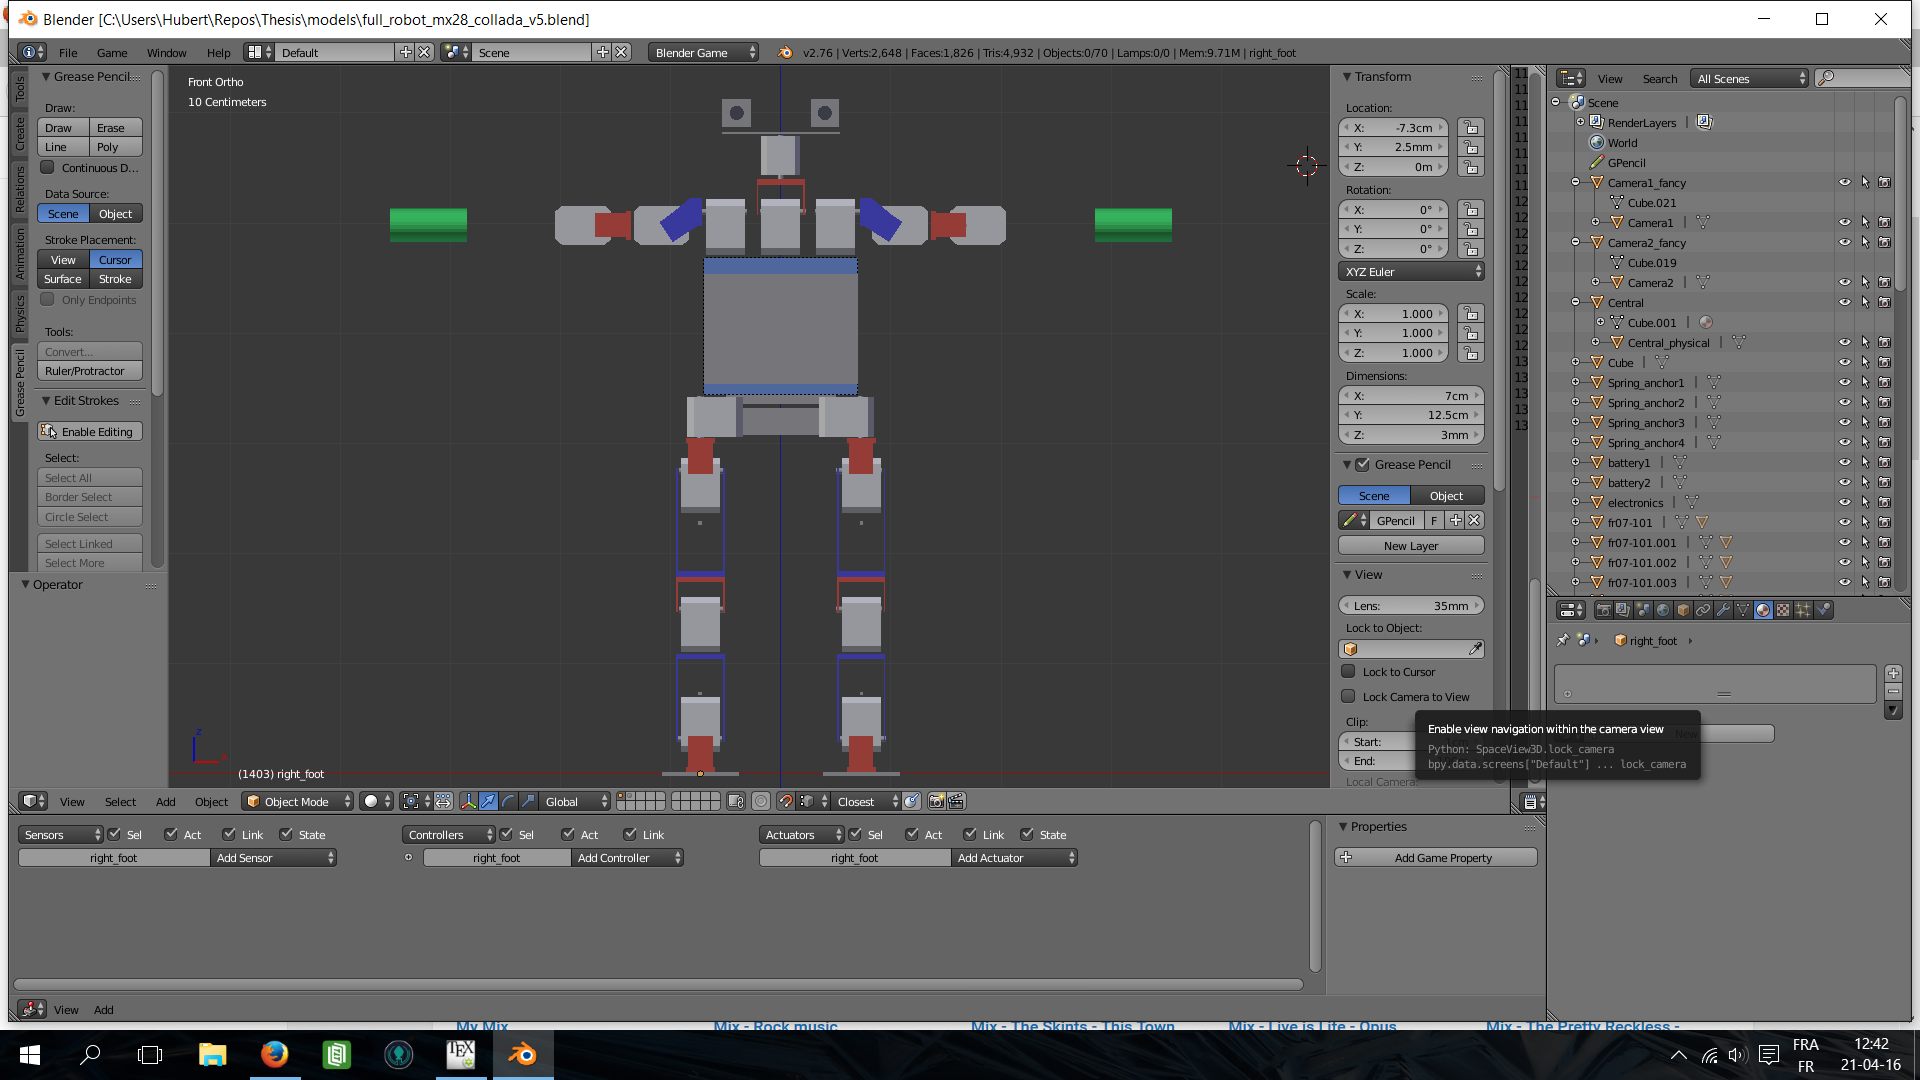
\includegraphics[width=0.6\textwidth]{figures/modelling_blender}
\caption[Front view of the robot's model at the end of the modelling in Blender]{Front view of the robot's model at the end of the modelling in Blender. The grey boxes represent the servos, the red pieces are standard Dynamixel frames, the blue are non-standard, the green cylinders are the hands.}
\label{fig:modelling_blender}
\end{figure}

\section{V-REP}
The model is finalized by :
\begin{itemize}
\item defining the mass and inertia of each piece(compiled in \cref{table:weights}) and enabling them for dynamic simulation.
\item adding joints between servos. For 2DOF joints, frame are used as intermediates.
\item adding vision sensors to simulate cameras.
\item adding scripts to simulate sensors (COG, accelerometers).
\item adding springs on the legs through the use of prismatic and spheric joints.
\end{itemize}

\subsection{Servos}
Servos are simulated by joints.

\subsection{Joints}
Spherical joint : 3DOF angular.

Prismatic joint : 1DOF linear.

Revolute joint : 1DOF angular.

\subsection{Sensors (accel, cog)}
The COG is computed through a script inside V-Rep, attached to a piece of the model and made available through the remote interface\cite{vrep_manual}.

\subsection{Springs}
Springs are simulated by prismatic and spherical joints.

An example of what the model looks like at the end of this process is visible on \cref{fig:modelling_vrep}.
\begin{figure}[htp]
\center
    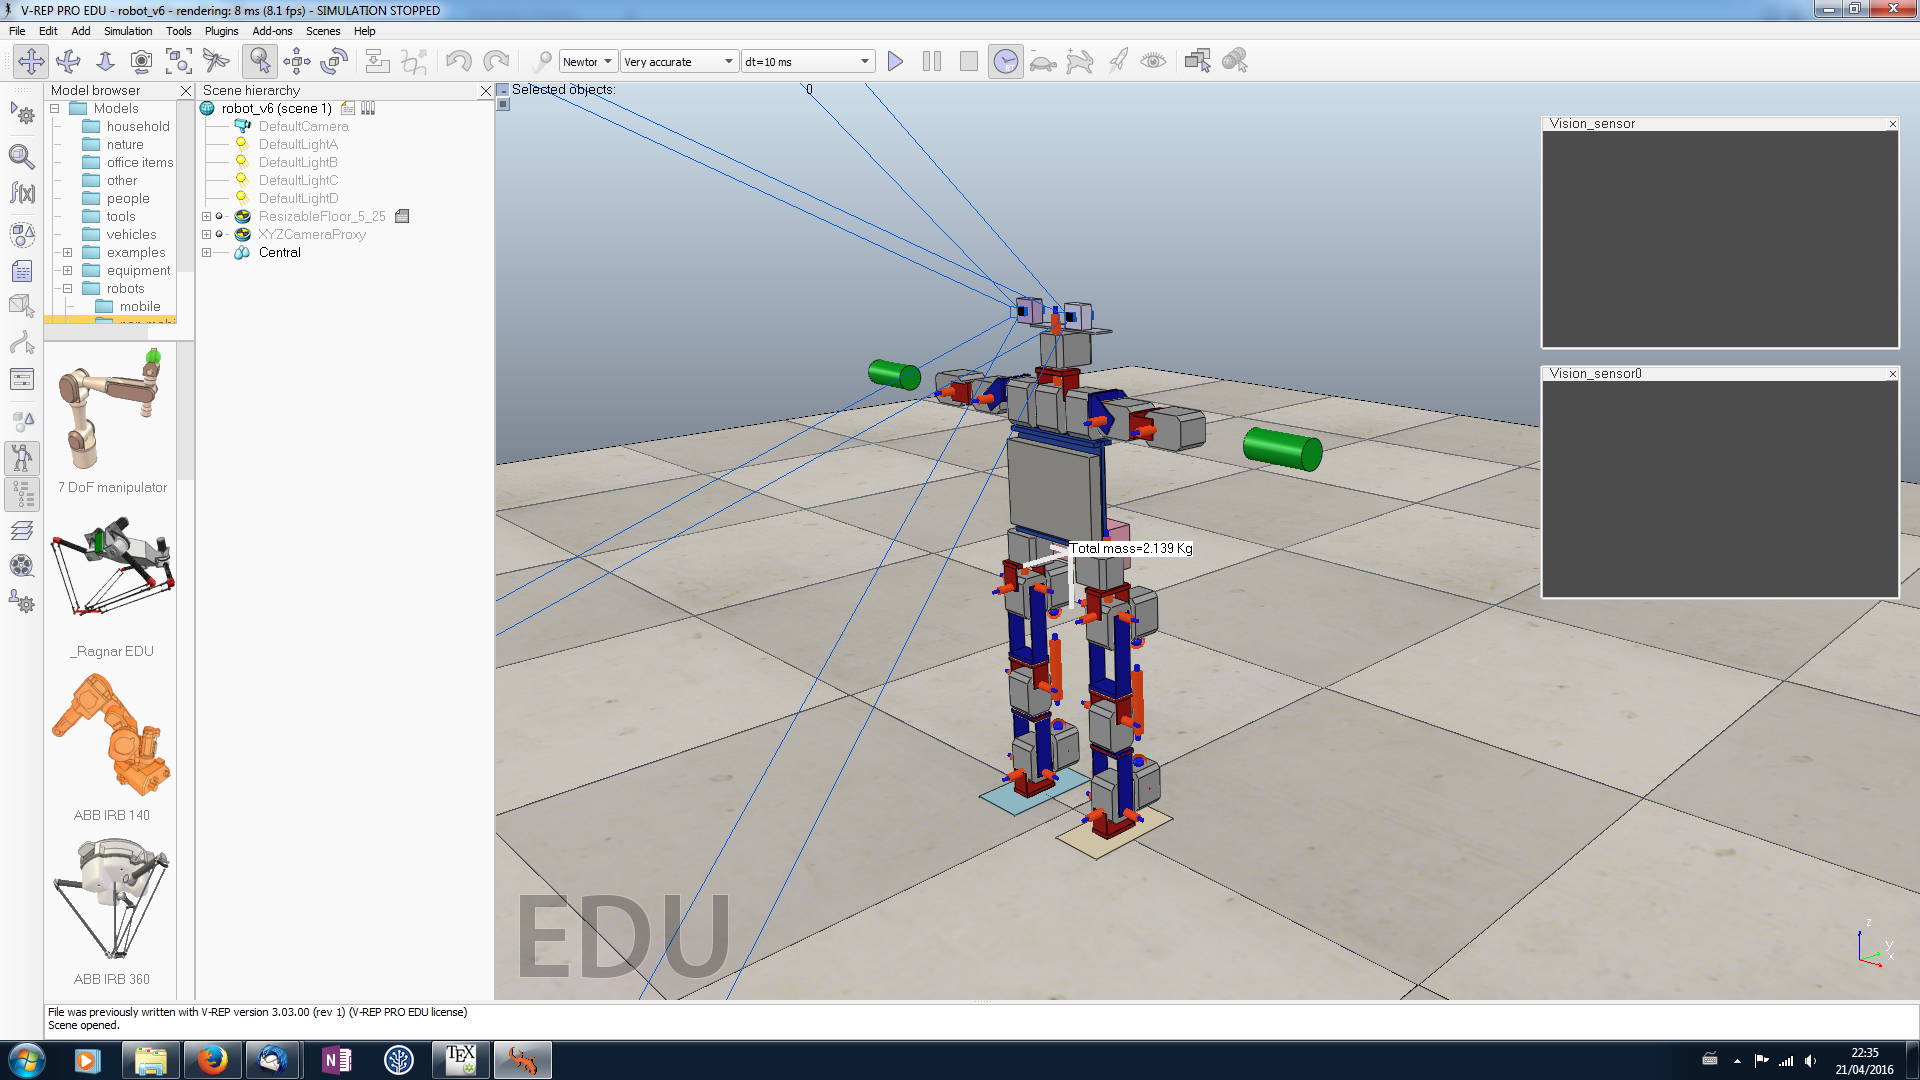
\includegraphics[width = 0.6\textwidth]{figures/modelling_vrep}
    \caption[View of the robot's model at the end of the modelling in V-REP]{View of the robot's model at the end of the modelling in V-REP.}
    \label{fig:modelling_vrep}
\end{figure}

\section{Simulation settings}